\documentclass[preprint,12pt,aps,pra,showkeys,amsmath,amssymb,superscriptaddress,floatfix]{revtex4-2}
\usepackage[T1]{fontenc}
\usepackage[utf8]{inputenc}
\usepackage{amsmath,amssymb,amsthm,mathtools,mathrsfs}
\usepackage{microtype,booktabs,enumitem}
\usepackage{xcolor,tikz,etoolbox}
\usepackage[skins,breakable]{tcolorbox}
\usepackage{needspace}
% Keep diagram geometry independent of REVTeX preprint body spacing.
\AtBeginEnvironment{tikzpicture}{\linespread{1}\selectfont}
\usetikzlibrary{arrows.meta,positioning,calc,fit,decorations.pathreplacing}
\usepackage{graphicx}
\usepackage{hyperref}

\definecolor{MMBlue}{RGB}{0,82,155}
\definecolor{MMOrange}{RGB}{200,80,0}
\tikzset{
 mmnode/.style={draw=MMBlue,rounded corners=2pt,fill=MMBlue!4,align=left,execute at begin node={\raggedright},text width=5cm,font=\fontsize{10}{12}\selectfont,inner sep=6pt},
 mmimport/.style={mmnode,draw=black!65,fill=black!4},
 mmcandidate/.style={mmnode,draw=MMOrange,dashed,fill=MMOrange!5},
 mmrejected/.style={mmnode,draw=black,densely dotted,fill=black!8},
 mmproof/.style={->,thick,MMBlue},
 mmflow/.style={->,semithick,black!70},
 mmrepair/.style={->,dashed,thick,MMOrange},
 mmcandidatearrow/.style={->,dashed,semithick,MMOrange},
 mmnote/.style={font=\scriptsize,fill=white,inner sep=2pt,align=center}}

\usepackage[section]{placeins}
\setlength{\emergencystretch}{3em}
\setlist{itemsep=3pt,topsep=4pt}
\newtheorem{theorem}{Theorem}[section]
\newtheorem{proposition}[theorem]{Proposition}
\newtheorem{lemma}[theorem]{Lemma}
\newtheorem{corollary}[theorem]{Corollary}
\theoremstyle{definition}
\newtheorem{definition}[theorem]{Definition}
\newtheorem{example}[theorem]{Example}
\theoremstyle{remark}
\newtheorem{remark}[theorem]{Remark}
% Avoid isolated statement headings and single-line paragraph fragments.
\BeforeBeginEnvironment{theorem}{\Needspace{6\baselineskip}}
\BeforeBeginEnvironment{definition}{\Needspace{5\baselineskip}}
\BeforeBeginEnvironment{proposition}{\Needspace{5\baselineskip}}
\BeforeBeginEnvironment{lemma}{\Needspace{5\baselineskip}}
\BeforeBeginEnvironment{corollary}{\Needspace{5\baselineskip}}
\clubpenalty=5000
\widowpenalty=5000
\newcommand{\R}{\mathbb R}\newcommand{\Z}{\mathbb Z}\newcommand{\N}{\mathbb N}
\newcommand{\Pa}{\operatorname{Pa}}\newcommand{\Desc}{\operatorname{Desc}}
\newcommand{\cl}{\operatorname{cl}}\newcommand{\cost}{\operatorname{cost}}
\newcommand{\status}{\operatorname{status}}
% Faculty cards: a visual rail groups the five faculties within one agent.
% The rail has no arrowhead and does not represent a proof dependency.
\newcommand{\mmfacultybadge}[1]{%
 \node[circle,draw=MMBlue,line width=1pt,fill=white,
 minimum size=7mm,inner sep=0pt,font=\sffamily\small\bfseries,text=MMBlue]
 at ([xshift=15pt,yshift=-15pt]frame.north west) {#1};}
\newcommand{\mmfacultyrail}{%
 \draw[MMBlue!80,line width=1pt]
 ([xshift=15pt,yshift=2pt]frame.north west)--
 ([xshift=15pt,yshift=-2pt]frame.south west);}
\newtcolorbox{mmfacultybox}[2]{enhanced,breakable,
 colback=MMBlue!4,colframe=MMBlue!4,boxrule=0pt,arc=3pt,
 left=39pt,right=9pt,top=4pt,bottom=4pt,
 before skip=2pt,after skip=2pt,
 fontupper=\small\linespread{1.1}\selectfont,
 overlay unbroken={\mmfacultyrail\mmfacultybadge{#1}},
 overlay first={\mmfacultyrail\mmfacultybadge{#1}},
 overlay middle={\mmfacultyrail},overlay last={\mmfacultyrail}}
\newcommand{\mmfaculty}[3]{%
 \begin{mmfacultybox}{#1}{#2}
 {\sffamily\bfseries\color{MMBlue}#2}\par\smallskip #3
 \end{mmfacultybox}}
\newcommand{\agent}[9]{%
 \Needspace{8\baselineskip}
 \subsubsection{#1}
 \noindent\textbf{Object.} #2\par
 \noindent\textbf{Role.} #3\par\smallskip
 \mmfaculty{E}{Ego}{#4}
 \mmfaculty{M}{Memory}{#5}
 \mmfaculty{I}{Intellect}{#6}
 \mmfaculty{S}{Sense}{#7}
 \mmfaculty{A}{Action}{#8}
 \smallskip\noindent #9\par}

\usepackage{longtable,array,calc}
\providecommand{\tightlist}{\setlength{\itemsep}{2pt}\setlength{\parskip}{0pt}}
\makeatletter
\def\frontmatter@abstract@produce{\par\addvspace{\frontmatter@preabstractspace}%
\begingroup\prep@absbox\unvbox\absbox\post@absbox\endgroup
\addvspace{\frontmatter@postabstractspace}}
\makeatother
\newcommand{\field}[2]{\par\smallskip\noindent\textbf{#1.} #2\par}
\setlength{\emergencystretch}{5em}
\AtBeginEnvironment{verbatim}{\small\linespread{1.0}\selectfont}


\hypersetup{colorlinks=true,linkcolor=MMBlue,urlcolor=MMBlue,pdfauthor={Dibakar Sigdel}}

\begin{document}

\title{Doob's L2 Maximal Inequality\\[4pt]\large An End-to-End Meta-Math Walkthrough}

\author{Dibakar Sigdel}

\affiliation{Mindverse Computing LLC, Lynnwood, WA 98087, USA}

\date{October 2026}

\begin{abstract}

Partition the first crossing of a threshold by its time. Conditional
expectation transfers that crossing value to the terminal absolute
value; integrating thresholds produces the \(L^2\) estimate. The report
presents the target theorem, declared imports, a dependency graph,
five-faculty node contracts, a continuous proof, a worked example, and a
hypothesis-repair audit. It is an authored mathematical exposition, not
a deployed-agent transcript or a formal proof-assistant certificate.

\end{abstract}\maketitle\linespread{1.12}\selectfont

\noindent\textbf{PS-04 / Probability and Stochastic Processes / Report v1}

\section{Target and import contract}

\begin{theorem}

For a real square-integrable martingale \((M_k,\mathcal F_k)_{k=0}^N\)
at a deterministic finite horizon, prove
\(\mathbb E[\max_{0\le k\le N}|M_k|^2]\le4\mathbb E|M_N|^2\). The
maximum includes the initial value, and the constant is independent of
\(N\).

\end{theorem}

\subsection{Foundations and permitted imports}

Use the tower and pull-out properties of conditional expectation,
\(|\mathbb E[Z\mid\mathcal F]|\le\mathbb E[|Z|\mid\mathcal F]\),
Cauchy--Schwarz, and Tonelli for nonnegative integrands. The tail
formula
\(\mathbb EZ^2=\int_0^\infty2\lambda\mathbb P(Z>\lambda)d\lambda\)
follows by integrating \(Z^2=\int_0^Z2\lambda d\lambda\) and applying
Tonelli. No optional-stopping theorem is needed for the proof.

\clearpage\section{Node interaction workflow}

\begin{center}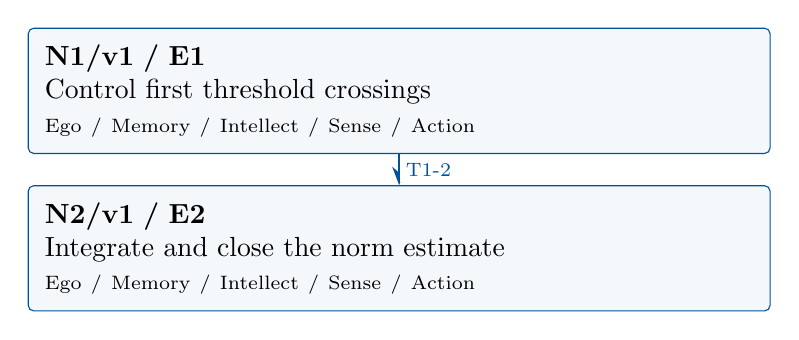
\begin{tikzpicture}[>=Stealth,x=1cm,y=1cm]

\node[mmnode,text width=9cm,minimum height=1.25cm] (N1) at (0,0.0) {\textbf{N1/v1 / E1}\\Control first threshold crossings\\{\scriptsize Ego / Memory / Intellect / Sense / Action}};

\node[mmnode,text width=9cm,minimum height=1.25cm] (N2) at (0,-2.0) {\textbf{N2/v1 / E2}\\Integrate and close the norm estimate\\{\scriptsize Ego / Memory / Intellect / Sense / Action}};

\draw[mmproof] (N1.south) -- node[mmnote,right] {T1-2} (N2.north);

\end{tikzpicture}\end{center}

Each box is one mathematical agent containing all five faculties. Blue
arrows carry the versioned exports listed below. The layout gives a
reading order; only drawn arrows assert dependencies. Diagnostic repair
is separate from the proof DAG.

\subsection{Versioned evidence-transfer ledger}

\begingroup\small\linespread{1.05}\selectfont

\Needspace{5\baselineskip}\field{T1-2: N1/E1/v1 to N2}{\(\lambda\mathbb P(Y^*>\lambda)\le\mathbb E[Y_N1_{\{Y^*>\lambda\}}]\).}

\field{Receiving activity}{N2.1}

\field{Compatibility}{E1/v1, finite horizon, and square integrability of every \(M_k\). Check:
\(Y^*\) is in \(L^2\) before division because
\((Y^*)^2\le\sum_{k=0}^N|M_k|^2\); this avoids a circular finiteness
argument.}

\endgroup

\clearpage\section{Agent roles and five-faculty activities}\begingroup\small\linespread{1.05}\selectfont\setlist{itemsep=1pt,topsep=2pt}

\subsection{N1/v1: Control first threshold crossings}

\field{Object and role}{Use disjoint first-crossing events, each measurable at its crossing
time. \textbf{Local obligation:}
\(\lambda\mathbb P(Y^*>\lambda)\le\mathbb E[Y_N1_{\{Y^*>\lambda\}}]\).}

\field{Inputs}{\(Y_k=|M_k|\), \(Y^*=\max_{0\le k\le N}Y_k\), and \(\lambda>0\).}

\mmfaculty{E}{Ego}{Publish E1/v1 only after establishing this obligation:
\(\lambda\mathbb P(Y^*>\lambda)\le\mathbb E[Y_N1_{\{Y^*>\lambda\}}]\).}

\mmfaculty{M}{Memory}{\(Y_k=|M_k|\), \(Y^*=\max_{0\le k\le N}Y_k\), and \(\lambda>0\). Retain
the stated assumptions and import versions.}

\mmfaculty{I}{Intellect}{Use disjoint first-crossing events, each measurable at its crossing
time.}

\mmfaculty{S}{Sense}{For each \(k\), \(\mathbb E[Y_N\mid\mathcal F_k]\ge Y_k\) follows from
the martingale property and conditional absolute-value inequality.}

\mmfaculty{A}{Action}{Carry out activities N1.1--N1.2 below, retaining each calculation and
construction as evidence.}

\smallskip\noindent\textbf{Numbered mathematical activities}

\begin{enumerate}[label=N1.\arabic*,leftmargin=3.4em]

\item Let \(A_k=\{Y_0\le\lambda,\ldots,Y_{k-1}\le\lambda,Y_k>\lambda\}\), with
the previous conditions empty for \(k=0\). These disjoint events lie in
\(\mathcal F_k\) and their union is \(\{Y^*>\lambda\}\). On \(A_k\),
\(Y_k>\lambda\).

\item By conditional expectation,
\(\mathbb E[Y_N1_{A_k}]=\mathbb E[\mathbb E(Y_N\mid\mathcal F_k)1_{A_k}]\ge\mathbb E[Y_k1_{A_k}]\ge\lambda\mathbb P(A_k)\).
Summing the finitely many inequalities gives the export.

\end{enumerate}

\field{Export E1/v1}{\(\lambda\mathbb P(Y^*>\lambda)\le\mathbb E[Y_N1_{\{Y^*>\lambda\}}]\).}

\field{Acceptance gate}{For each \(k\), \(\mathbb E[Y_N\mid\mathcal F_k]\ge Y_k\) follows from
the martingale property and conditional absolute-value inequality.}

\field{Targeted repair}{If the whole crossing event is treated as measurable at every time,
partition it by first-crossing time before applying conditional
expectation. Withhold this export and recheck its descendants after a
versioned correction.}

\clearpage

\subsection{N2/v1: Integrate and close the norm estimate}

\field{Object and role}{Integrate the tail bound and apply Cauchy--Schwarz, justifying division
by the maximal norm. \textbf{Local obligation:}
\(\|Y^*\|_2\le2\|M_N\|_2\), hence the claimed squared bound.}

\field{Inputs}{E1/v1, finite horizon, and square integrability of every \(M_k\).
Incoming proof exports: E1/v1 at N2.1.}

\mmfaculty{E}{Ego}{Publish E2/v1 only after establishing this obligation:
\(\|Y^*\|_2\le2\|M_N\|_2\), hence the claimed squared bound.}

\mmfaculty{M}{Memory}{E1/v1, finite horizon, and square integrability of every \(M_k\).
Incoming proof exports: E1/v1 at N2.1. Retain the stated assumptions and
import versions.}

\mmfaculty{I}{Intellect}{Integrate the tail bound and apply Cauchy--Schwarz, justifying division
by the maximal norm.}

\mmfaculty{S}{Sense}{\(Y^*\) is in \(L^2\) before division because
\((Y^*)^2\le\sum_{k=0}^N|M_k|^2\); this avoids a circular finiteness
argument.}

\mmfaculty{A}{Action}{Carry out activities N2.1--N2.2 below, retaining each calculation and
construction as evidence.}

\smallskip\noindent\textbf{Numbered mathematical activities}

\begin{enumerate}[label=N2.\arabic*,leftmargin=3.4em]

\item The finite-sum bound makes \(A=\|Y^*\|_2\) finite. Multiply E1 by \(2\)
and integrate \(\lambda\) over \((0,\infty)\). The tail formula and
Tonelli give
\(A^2\le2\int_0^\infty\mathbb E[Y_N1_{\{Y^*>\lambda\}}]d\lambda=2\mathbb E[Y_NY^*]\).

\item Cauchy--Schwarz bounds the final expression by \(2\|Y_N\|_2 A\). If
\(A=0\), the conclusion is immediate. Otherwise divide by \(A\) to
obtain \(A\le2\|Y_N\|_2\) and square. The factor four and horizon
independence follow.

\end{enumerate}

\field{Export E2/v1}{\(\|Y^*\|_2\le2\|M_N\|_2\), hence the claimed squared bound.}

\field{Acceptance gate}{\(Y^*\) is in \(L^2\) before division because
\((Y^*)^2\le\sum_{k=0}^N|M_k|^2\); this avoids a circular finiteness
argument.}

\field{Targeted repair}{If division is performed before maximal integrability is known, first
use the finite sum of squared values, then handle the zero-norm case
separately. Withhold this export and recheck its descendants after a
versioned correction.}

\endgroup\clearpage\section{Continuous mathematical proof}\label{sec:proof}

\subsection{N1 --- Control first threshold
crossings}\label{n1-control-first-threshold-crossings}

\begin{enumerate}
\def\labelenumi{\arabic{enumi}.}
\item
  \textbf{N1.1.} Let
  \(A_k=\{Y_0\le\lambda,\ldots,Y_{k-1}\le\lambda,Y_k>\lambda\}\), with
  the previous conditions empty for \(k=0\). These disjoint events lie
  in \(\mathcal F_k\) and their union is \(\{Y^*>\lambda\}\). On
  \(A_k\), \(Y_k>\lambda\).
\item
  \textbf{N1.2.} By conditional expectation,
  \(\mathbb E[Y_N1_{A_k}]=\mathbb E[\mathbb E(Y_N\mid\mathcal F_k)1_{A_k}]\ge\mathbb E[Y_k1_{A_k}]\ge\lambda\mathbb P(A_k)\).
  Summing the finitely many inequalities gives the export.
\end{enumerate}

\subsection{N2 --- Integrate and close the norm
estimate}\label{n2-integrate-and-close-the-norm-estimate}

\begin{enumerate}
\def\labelenumi{\arabic{enumi}.}
\item
  \textbf{N2.1.} The finite-sum bound makes \(A=\|Y^*\|_2\) finite.
  Multiply E1 by \(2\) and integrate \(\lambda\) over \((0,\infty)\).
  The tail formula and Tonelli give
  \(A^2\le2\int_0^\infty\mathbb E[Y_N1_{\{Y^*>\lambda\}}]d\lambda=2\mathbb E[Y_NY^*]\).
\item
  \textbf{N2.2.} Cauchy--Schwarz bounds the final expression by
  \(2\|Y_N\|_2 A\). If \(A=0\), the conclusion is immediate. Otherwise
  divide by \(A\) to obtain \(A\le2\|Y_N\|_2\) and square. The factor
  four and horizon independence follow.
\end{enumerate}

\hfill$\square$

\section{Worked orchestration}

For a symmetric random walk with two increments and \(M_0=0\), paths
\(++\) and \(--\) have squared maximum four, while \(+-\) and \(-+\)
have squared maximum one. Thus \(\mathbb E(Y^*)^2=(4+4+1+1)/4=5/2\). The
terminal second moment is two, and \(5/2\le4\cdot2=8\). The bound
controls the whole path, not merely its endpoint.

\subsection{Boundary and hypothesis audit}

Adaptation alone is insufficient. The deterministic process
\(M_0=1,M_1=0\) is adapted and square-integrable but not a martingale.
Its maximal square is one while its terminal square is zero,
contradicting the claimed inequality without the martingale hypothesis.

\section{Illustrative failure and repair}

The following is an authored diagnostic scenario. Changed assumptions
define a new contract; they do not retroactively prove the original
statement.

\subsection{Rejected argument, diagnosis, and correction}
\textbf{Rejected N1 inequality:}
\(\mathbb E[Y_N\mid\mathcal F_k]\ge Y_k\) holds for any adapted process.
The deterministic decay example disproves it. \textbf{Repair:} derive it
from \(M_k=\mathbb E[M_N\mid\mathcal F_k]\) and the conditional
absolute-value inequality, exactly as the import contract allows for a
martingale. Recheck the crossing bound and integrated estimate under
those hypotheses.

\subsection{Publication and reuse}
The corrected export retains its explicit assumptions. A hypothetical
revision receives a new version, and each consuming activity is
rechecked; this scenario is not a recorded runtime event. \textbf{Next
direction:} Use the inequality to control convergence of martingale
approximations or construct stochastic integrals in \(L^2\).

\par\medskip\begingroup\small\linespread{1.0}\selectfont\noindent\textbf{Provenance.} This authored proof is complete relative to its declared imports. Reuse
each export with its assumptions, proof, and version. The original
Markdown remains available for comparison.
\par\endgroup

\par\smallskip\begingroup\small\linespread{1.0}\selectfont\noindent\textbf{Further reading.} \href{https://stanford.edu/~montanar/TEACHING/Stat310A/lnotes.pdf}{Amir
Dembo, Probability Theory: STAT310/MATH230 notes} for measure-theoretic
probability and limit arguments;
\href{https://web.stanford.edu/class/stats310c/syllabus.html}{Stanford
STAT310C syllabus and lecture materials} for martingale inequalities and
stopping theorems. The versions and proofs used in this collection are
stated explicitly.\par\endgroup

\end{document}
